\chapter{Criptografía Básica} \label{ch:primer-capitulo}

    En este capítulo establecemos los fundamentos esenciales de la Criptografía. Estos conceptos y herramientas servirán como base para comprender los aspectos más avanzados de la seguridad de la información en capítulos posteriores. Para su elaboración, se han utilizado principalmente \cite{cryptoSchool} y \cite{artDH}.
    
    \section{Introducción}
    
     Desde la antigüedad, la criptografía ha sido utilizada para mantener la privacidad y la confidencialidad en la comunicación de mensajes importantes. Hoy en día, se ha convertido en una herramienta crucial para proteger los datos sensibles en sistemas informáticos y en la comunicación en línea.

    En este capítulo, se abordarán algunos conceptos fundamentales de la criptografía moderna, incluyendo los sistemas criptográficos simétricos y asimétricos, técnicas de intercambios de claves y los algoritmos de cifrado y descifrado tales como AES o RSA.

    La principal tarea que tiene la criptografía es la trasmisión segura de información. Siguiendo la tradición \cite{cryptoSchool}, se suele explicar que un usuario A, denominado Alice, quiere enviar un mensaje secreto a un destinatario B, llamado Bob. En este escenario, también se encuentra Eva, que quiere enterarse del mensaje secreto que envía Alice, y estará atenta al canal de comunicación que utilicen Alice y Bob, para interceptar todos sus mensajes.

    Para conseguir esto, Alice tendrá que encriptar su mensaje $x$ con una clave $K$ y enviarle a Bob el resultado $y = enc_{K}(x)$. Por tanto, luego Bob deberá desencriptar el mensaje encriptado $y$ con su propia clave $S$, para obtener el mensaje original $x = dec_{S}(y)$.

    Obviamente surgen diversas dudas ante esta situación, tales como: ¿Cómo puede hacerle llegar Alice a Bob la clave necesaria para desencriptar el mensaje? ¿Qué métodos son ``mejores'' para encriptar el mensaje? O en el peor de los casos, ¿qué pasaría si Eva averigua la clave que están usando?

    Volviendo al escenario planteado, está claro que, a priori, nos da igual que Eva consiga el mensaje encriptado, siempre y cuando no sea capaz de desencriptarlo. Por tanto, Alice debería utilizar una función que no sea fácil de desencriptar, ya que su mensaje sería vulnerable. Llamamos a esta función, función unidireccional.
    
    \begin{definicion} \cite{cryptoSchool} 
        Una \textit{función unidireccional} es una función $f$ tal que dado $x$, $f(x) = y$ es fácil de computar, pero que dado $y$, sea dificil encontrar un $x$ tal que $f(x) = y$. Si además, Bob tiene algún secreto $S$, el cual le permite encontrar $x$ a partir de $y$ de manera sencilla, diremos que $f$ es una \textit{función trampilla}.
    \end{definicion}

    \begin{ejemplo} \cite{cryptoSchool}
        Sea $x = (p,q)$ con $p$ y $q$ primos tal que $p < q$ y $f(x) = p \cdot q$. \\
        Es fácil multiplicar ambos números primos para obtener un valor $N$, pero es muy dificil, a nivel computacional, obtener los primos $p$ y $q$ a partir del valor $N$. De hecho, no se conoce ninguna función trampilla para esta $f$. Ésta es la función unidireccional utilizada en el algoritmo RSA, que se explicará más adelante.
    \end{ejemplo}

    En realidad, que Eva ``rompa el sistema'', no tiene que significar necesariamente que sea capaz de descifrar el mensaje de manera completa. Podría simplemente limitarse a desencriptar una pequeña parte del mensaje, como por ejemplo conocer el idioma en el que está escrito; o incluso buscar palabras clave, como podrían ser ``bomba'' o ``Mastercard'', entre otras posibilidades. Obviamente, debe ser inviable poder recuperar tanto el mensaje $x$, como la clave de Bob $S$, a partir del mensaje $y$. 
    
    Por otro lado, otro tipo de ataque sería que Eva consiga ver los valores de distintas $enc_{k}(x)$ para varios $x$ diferentes. Este tipo de ataque se denomina \textit{chosen plaintext attack} (CPA). Entre los diversos objetivos del ataque, el primero que se nos ocurre es recuperar la clave secreta que se utiliza en el cifrado. Por tanto, una característica deseable es la indistinguibilidad.

    \begin{definicion} \cite{cryptoSchool}
        Definimos \textit{indistinguibilidad} en este contexto como la capacidad de no poder distinguir a partir de una imagen $enc_{k}(x)$, su preimagen $x$ asociada. 
    \end{definicion}
    
    Para entender este concepto, supongamos que Eva envía dos textos planos distintos y recibe uno de ellos desencriptado, $y_{0}$, de tal forma que ha sido seleccionado entre los dos textos planos con igual probabilidad. En esta situación, Eva debe determinar cual de los dos textos originales ha sido desencriptado, basándose no solo en la aleatoriedad. Así, la indistinguibilidad es la resistencia a este tipo de ataque, de manera que Eva no pueda saber cúal ha sido el texto original escogido. Procedemos a continuación a la explicación de uno de los algoritmos más populares de toda la criptografía simétrica, el algoritmo AES.

    \section{Advanced Encryption Standard (AES)}

    El estándar de cifrado avanzado (AES) es un esquema de cifrado por bloques creado en Bélgica pero adoptado como un estándar de cifrado por el gobierno de los Estados Unidos. Tras ser anunciado por el \textit{Instituto Nacional de Estándares y Tecnología} (NIST) en $2001$, se estandarizó finalmente en Mayo de $2002$. Desde $2006$, AES es uno de los algoritmos más populares usados en criptografía simétrica.

    \subsection{Historia de AES}

    A principios de los años $70$, un equipo de International Business Machines desarrolló un criptosistema que se conoció como \textit{Estándar de Cifrado de Datos} (DES). La \textit{National Bureau of Standards} (NBS) de EE.UU lo publicó en el $1977$ como estandar para la criptografía del gobierno estadounidense, en particular para documentos sensibles pero no clasificados. Como consecuencia, cualquier sistema de software o hardware con capacidades criptográficas que se ofreciera al gobierno estadounidense, tenía que estar basado en DES. 
    
    Dado que las ventas a entidades gubernamentales pueden resultar altamente rentables, cualquier compañía que deseara participar en este mercado, debía emplear DES. Como resultado, su uso se generalizó rápidamente. A lo largo de los años, se desarrollaron diversos ataques contra DES, sobre todo basados en el criptoanálisis diferencial y lineal. En respuesta a esto y ante la preocupación por su reducido espacio de claves, DES se reforzó triplicando su número de ``rondas'', convirtiéndose así en triple-DES o $3$-DES.

    Desde el principio, los expertos albergaron sospechas, nunca confirmadas, de que la \textit{National Security Agency} (NSA) podría haber construido una función trampilla para DES que le permitiera descifrar mensajes. Ya en $1981$, se advirtió que la agencia NSA era capaz de romper DES utilizando un texto plano probable. Se decía que el principal hardware criptoanalítico implicado consistía en cuatro ordenadores CRAY-$1$ y que el análisis duraba menos de $24$ horas de media.

    Finalmente, en $1998$ \textit{Electronic Frontier Foundation} (EFF) presentó su  US\$ $250,000$ DES breaker. Así, DES estaba muerto para la mayoría de casos prácticos, aunque el estandar no se retiró hasta $2005$. 
    
    Previamente, en $1997$, la agencia sucesora a NBS, US NIST, abrió una competición para crear AES y reemplazar a DES. Los requisitos eran un cifrado por bloques de $128$ bits, y longitudes de clave posibles de $128$, $192$ y $256$ bits. Como era de esperar, las especificaciones eran bastante más precisas que las de su competición de $1973$, que condujo a la adopción de DES. 
    
    Se presentaron a NIST $15$ candidatos, pero se redujeron a una pequeña lista de $5$ sistemas para Agosto de $1999$. Estos candidatos eran:

    \begin{enumerate}
        \item \textbf{MARS}: desarrollado por Don Coppersmith de IBM, uno de los creadores principales de DES.
        \item \textbf{RC6}: desarrollado por Ron Rivest y $3$ colaboradores de RSA Laboratories.
        \item \textbf{Serpent}: desarrollado por Anderson, Biham y Knudsen.
        \item \textbf{Twofish}: desarrollado por la empresa Counterpane de Bruce Schneier.
        \item \textbf{Rijndael}: desarrollado por dos criptógrafos belgas llamados Joan Daemen y Vincent Rijmen.
    \end{enumerate}

    En Octubre del año $2000$, NIST anunció que el ganador era Rijndael. Se esperaba que este sistema fuera seguro durante al menos $30$ años.

    Por lo general, se alabó al NIST por realizar un procedimiento abierto y bien documentado. Uno de sus requisitos que estableció era demostrar de manera creíble que no existían funciones trampilla ocultas, aliviando así algunas de las preocupaciones que habían surgido durante la estandarización del DES en $1977$.

    Las características que aseguraron el primer puesto para Rijndael son la seguridad, resistencia ante todos los ataques conocidos y la eficiencia en amplia variedad de plataformas. Además, se caracteriza por una descripción algebraica simple con pocas características inexplicables, lo que hace altamente improbable la existencia de una función trampilla. Hasta el año $2023$, no se ha identificado ningún ataque efectivo contra él.

    \subsection{Descripción de AES}
    
    AES cifra un mensaje de $128$ bits utilizando una clave de $128$, $192$ o $256$ bits, que se distinguen por denominaciones como AES-$128$. Es un cifrado iterado en el que una secuencia de cuatro operaciones se aplica un número determinado de veces. Consta de $10$ rondas cuando la longitud de clave es de $128$, $12$ rondas con longitud $192$ y $14$ rondas con longitud $256$. Para la totalidad de la explicación, trabajaremos con AES-$128$.
    
    En cada ronda realiza cuatro operaciones, salvo que en la última ronda se omite una de ellas y en la primera se añade otra. Cada operación convierte una palabra de $128$ bits en otra de $128$ bits, es decir, se mantiene la longitud. Para describir las operaciones, cada palabra de $128$ bits (o estado en AES) es tratada como una matriz $4x4$ donde cada elemento $a_{ij}$ con $i,j = 0, 1, 2, 3$, es un byte de $8$ bits de la siguiente forma:
    \begin{equation}
        \begin{bmatrix}
            a_{00} & a_{01} & a_{02} & a_{03} \\
            a_{10} & a_{11} & a_{12} & a_{13} \\
            a_{20} & a_{21} & a_{22} & a_{23} \\
            a_{30} & a_{31} & a_{32} & a_{33} \\
        \end{bmatrix}
    \end{equation}
    
    Las operaciones y etapas de AES se explican y se muestran a continuación:
    \begin{enumerate}
        \item \textbf{SUBBYTES}: sustituye cada byte por otro valor.
        \item \textbf{SHIFTROWS}: permuta los bytes de cada fila.
        \item \textbf{MIXCOLUMNS}: aplica una transformación lineal a cada columna.
        \item \textbf{ADDROUNDKEY}: añade una clave a toda la matriz.
    \end{enumerate}
    
    \begin{figure}[H]
        \centering
        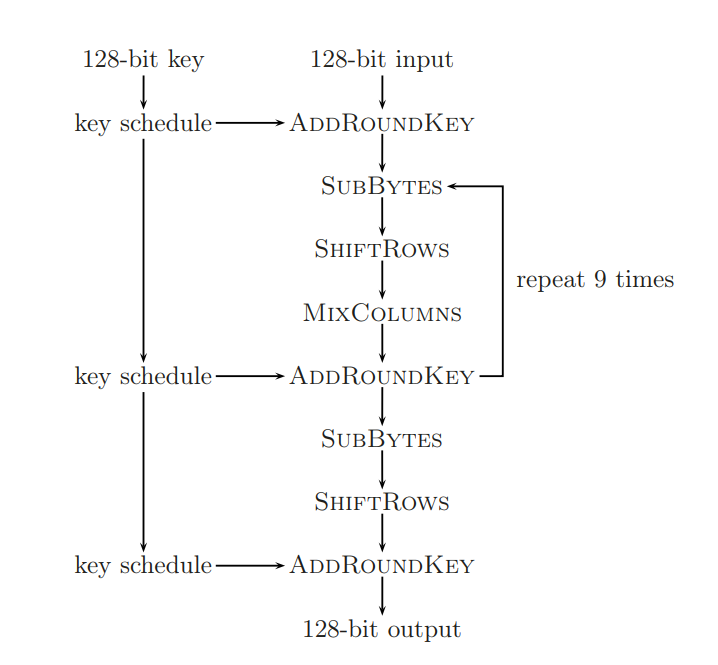
\includegraphics[width=0.7\textwidth, height=0.7\textheight, keepaspectratio]{AES}
        \caption{Rondas de AES-$128$ \cite{cryptoSchool}.}
        \label{fig:1.1}
    \end{figure}
    
    Seguidamente, vamos a proceder a explicar en más detalle las distintas operaciones que constituyen AES. A medida que avancemos en este documento, también exploraremos otros sistemas de cifrado como RSA o Merkle-Hellman, entre otros. No obstante, de la elegante explicación algebraica que se presenta a continuación, destaca la sorprendente eficacia del álgebra en el campo de la criptografía.

    \subsection{Operaciones de AES}

    La unidad básica de procesamiento es el byte, formado por $8$ bits.
    \begin{equation}
        a = (a_{7}, a_{6}, a_{5}, a_{4}, a_{3}, a_{2}, a_{1}, a_{0}) \in \{0, 1\}^{8}
    \end{equation}
    Las operaciones básicas de los bytes son la suma y la multiplicación. Las definimos de la siguiente forma:
    \begin{itemize}
        \item \textbf{Suma}. Sean $a, b, c \in \{0, 1\}^{8}$, la suma de dos bytes es la suma bit a bit módulo $2$:
        \begin{equation}
            c_{i} = (a_{i} + b_{i}) \text{ mod } 2 \text{ , con } i = 0, ... , 7
        \end{equation}
        \begin{ejemplo}
            Por ejemplo, sea $a = (1, 0, 0, 1, 1, 0, 1, 1)$ y $b = (1, 1, 0, 0, 1, 1, 0, 1)$, entonces: 
            \begin{equation}
                c = a + b = (0, 1, 0, 1, 0, 1, 1, 0)
            \end{equation}
        \end{ejemplo}
        \item \textbf{Producto}. Para el producto, consideramos que el byte $a$ está representando el siguiente polinomio:
        \begin{equation}
            a_{7}t^{7} + a_{6}t^{6} + \ldots + a_{1}t + a_{0} \in \mathbb{F}_{2}[t]
        \end{equation}
        De esta forma, el producto $p = a \cdot b$ se calcula multiplicando ambos polinomios, obteniendo un polinomio de grado $14$ como máximo. Aunque ahora tenemos un problema obvio, ya que el resultado obtenido tiene $15$ bits pero la operación debe devolver al final solo $8$. Para solucionar esto, lo que haremos será reducir módulo un polinomio de grado $8$. De hecho, en AES trabajamos en el campo finito $\mathbb{F}_{256}$ definido por el polinomio irreducible:
        \begin{equation}
            m = t^{8} + t^{4} + t^{3} + t + 1 \in \mathbb{F}_{2}[t]
        \end{equation}
        Por tanto, $p$ mod $m \in \mathbb{F}_{2}[t]/(m) = \mathbb{F}_{2^{8}} = \mathbb{F}_{256}$, volviendo de nuevo al grado máximo de $8$ bits que nos da el resultado final del producto:
        \begin{align}
            c = a_{7}t^{7} + a_{6}t^{6} + &a_{5}t^{5} + a_{4}t^{4} + a_{3}t^{3} + a_{2}t^{2} + a_{1}t + a_{0} \in \mathbb{F}_{256} \\
            &\text{con } a_{i} \in \{0, 1\} \text{, } i = 0, ... , 7
        \end{align}
        Veamos un ejemplo que nos clarifique los conceptos vistos.
        \begin{ejemplo}
            Sea $a = (1, 0, 0, 1, 1, 0, 1, 1)$ y $b = (1, 1, 0, 0, 1, 1, 0, 1)$ los mismos valores de antes. Ahora, sin embargo, representan los siguientes polinomios respectivamente:
            \begin{align}
                a = t^{7} + t^{4} + t^{3} + t + 1 \in \mathbb{F}_{2}[t] \\
                b = t^{7} + t^{6} + t^{3} + t^{2} + 1 \in \mathbb{F}_{2}[t]
            \end{align}
            El producto de estos polinomios es:
            \begin{equation}
                p = t^{14} + t^{13} + t^{11} + t^{10} + t^{8} + t^{6} + t^{5} + t^{3} + t^{2} + t + 1 \in \mathbb{F}_{2}[t]
            \end{equation}
            Recordemos que el polinomio irreducible es:
            \begin{equation}
                m = t^{8} + t^{4} + t^{3} + t + 1 \in \mathbb{F}_{2}[t]
            \end{equation}
            A continuación, calculamos $p$ mod $m$, esto es, dividimos $p$ entre $m$ y nos quedamos con el resto, obteniendo:
            \begin{equation}
                p = (t^{6} + t^{5} + t^{3}) \cdot m + (t^{4} + t^{2} + t + 1) \in \mathbb{F}_{2}[t]
            \end{equation}
            Finalmente, fijándonos en el resto, obtenemos que este polinomio es la representación de $c = (0, 0, 0, 1, 0, 1, 1, 1)$.
        \end{ejemplo}
    \end{itemize}

    \subsubsection{SubBytes}

    La operación SubBytes de AES aplica una transformación a cada byte de la matriz $4x4$. Es por ello que el apartado anterior define las dos operaciones principales que vamos a utilizar, la suma y el producto. Estas operaciones las realizamos a partir de dos bytes, obteniendo otro byte como resultado. El problema es que en SubBytes, solo tenemos un byte de entrada. Para solucionar esto, haremos uso de la inversa.

    Como $\mathbb{F}_{256}$ es un cuerpo, todo elemento no nulo $a \in \mathbb{F}^{x}_{256}$ tiene un inverso $a^{-1} \in \mathbb{F}^{x}_{256}$. Este elemento inverso se puede calcular mediante el Algoritmo Extendido de Euclides. Definimos esta función en todo $\mathbb{F}_{256}$ simplemente enviando cero a si mismo:
    \[
    \text{inv(}a\text{)} = 
    \left\{
        \begin{array}{l}
            a^{-1} \text{, si } a \neq 00 \\
            00 \text{, si } a = 00 
        \end{array}
    \right.
    \]
    donde $00 = (0, 0, 0, 0, 0, 0, 0, 0)$. Entendamos lo explicado en el siguiente ejemplo.
    \begin{ejemplo} \cite{cryptoSchool}
        Tomando los valores de los ejemplos vistos previamente, el Algoritmo Extendido de Euclides nos da la siguiente igualdad:
        \begin{equation}
            (t^{7} + t^{3}) \cdot a + (t^{6} + t^{3} + t^{2} + t + 1) \cdot m = 1 \text{, en } \mathbb{F}_{2}[t]
        \end{equation}
        De hecho, como gcd($a,m$) = $1$, entonces:
        \begin{equation}
            \text{inv(}a\text{)} = (1, 0, 0, 0, 1, 0, 0, 0) \text{ en } \mathbb{F}_{256}.
        \end{equation}
    \end{ejemplo}

    AES utiliza una estructura algebraica similar, aunque diferente, sobre los bytes, llamada el anillo $R =  \mathbb{F}_{2}[t]/(t^{8}+1)$. Esta estructura no es un cuerpo, ya que $t^{8}+1 = (t+1)^{8}$ no es irreducible en $\mathbb{F}_{2}[t]$. Por tanto, ahora un byte $a$ representa al elemento:
    \begin{equation}
        a_{7}t^{7} + a_{6}t^{6} + a_{5}t^{5} + a_{4}t^{4} + a_{3}t^{3} + a_{2}t^{2} + a_{1}t + a_{0} \text{ en } R
    \end{equation}
    La suma, nuevamente, es la suma de bits módulo dos (o XOR), por lo que es válido en R. En la multiplicación, también se lleva a cabo el producto de polinomios, para luego reducir su grado tomando módulo con un polinomio de grado $8$, solo que en este caso, este polinomio de reducción es $m = t^{8}+1$. Esta reducción es particularmente sencilla ya que corresponde a dividir la parte superior e inferior del polinomio producto $p$ con tamaño $16$ bits, en dos partes que denominaremos $c_{1}$ y $c_{0}$ respectivamente, de tamaño $8$ bits cada una, para luego sumarlas y obtener el resultado final. Veamos esta idea en un ejemplo que nos resulte claro.

    \begin{ejemplo} 
        Tomando $a = (1, 0, 0, 1, 1, 0, 1, 1)$ y $b = (1, 1, 0, 0, 1, 1, 0, 1)$ los mismos valores previos, realizamos la multiplicación de los polinomios y obtenemos el mismo resultado anterior:
        \begin{equation}
            p = t^{14} + t^{13} + t^{11} + t^{10} + t^{8} + t^{6} + t^{5} + t^{3} + t^{2} + t + 1
        \end{equation}
        Recordemos ahora que el polinomio irreducible es:
        \begin{equation}
            m = t^{8} + 1
        \end{equation}
        Por tanto, aplicando ahora reducción de $p$ módulo $m$, obtendríamos lo siguiente:
        \begin{equation}
            p = (t^{6} + t^{5} + t^{3} + t^{2} + t + 1) \cdot m + t 
        \end{equation}
        Por tanto, el resultado final es $c = (0, 0, 0, 0, 0, 0, 1, 0)$, ya que debemos centrarnos solo en el resto. No obstante, lo particular de este polinomio irreducible es que es más fácil su cálculo, ya que podemos dividir el polinimio $p$ en dos partes, que hemos denominado $c_{1}$ y $c_{0}$. Esta idea se expresa en la siguiente igualdad:
        \begin{equation}
            p = c_{1} \cdot t^{8} + c_{0}
        \end{equation}
        Así, para calcular cada $c_{i}$, debemos dividir del polinomio $p$ con tamaño $16$ bits, en dos mitades con $8$ bits cada una, de tal forma que obtenemos:
        \begin{align}
            c_{1} = (0, 1, 1, 0, 1, 1, 0, 1) \\
            c_{0} = (0, 1, 1, 0, 1, 1, 1, 1)
        \end{align}
        Para finalizar, solo debemos sumar ambas $c_{i}$ usando la suma en $R$ y obtendremos el resultado final $c = (0, 0, 0, 0, 0, 0, 1, 0)$, que coincide con el que habíamos obtenido.
    \end{ejemplo}
    
    Tras haber explicado todo esto, cabe mencionar que en AES, realmente sólo se realiza el producto en $R$ por el polinomio fijo $t_{1}$, y solo se suma el polinomio $t_{0}$. Estos son:
    \begin{align}
        &t_{1} = (0, 0, 0, 1, 1, 1, 1, 1) = t^{4} + t^{3} + t^{2} + t + 1 \\
        &t_{0} = (0, 1, 1, 0, 0, 0, 1, 1) = t^{6} + t^{5} + t + 1 
    \end{align}
    Al ser $t_{1}$ invertible módulo $t^{8} + 1$, la multiplicación por $t_{1}$ corresponde a una transformación lineal invertible sobre $\mathbb{F}_{2}$. Así, para un byte $a$, debemos aplicar:
    \begin{equation}
        c = t_{1} \cdot b + t_{0}
    \end{equation}
    donde $b =$ inv($a$), visto previamente. Esto también puede ser descrito por una transformación lineal de la siguiente forma:
    \begin{equation}
        \begin{bmatrix}
            c_{7} \\
            c_{6} \\
            c_{5} \\
            c_{4} \\
            c_{3} \\
            c_{2} \\
            c_{1} \\
            c_{0} \\
        \end{bmatrix}
        =
        \begin{bmatrix}
            1 & 1 & 1 & 1 & 1 & 0 & 0 & 0 \\
            0 & 1 & 1 & 1 & 1 & 1 & 0 & 0 \\
            0 & 0 & 1 & 1 & 1 & 1 & 1 & 0 \\
            0 & 0 & 0 & 1 & 1 & 1 & 1 & 1 \\
            1 & 0 & 0 & 0 & 1 & 1 & 1 & 1 \\
            1 & 1 & 0 & 0 & 0 & 1 & 1 & 1 \\
            1 & 1 & 1 & 0 & 0 & 0 & 1 & 1 \\
            1 & 1 & 1 & 1 & 0 & 0 & 0 & 1 \\
        \end{bmatrix}
        \cdot
        \begin{bmatrix}
            b_{7} \\
            b_{6} \\
            b_{5} \\
            b_{4} \\
            b_{3} \\
            b_{2} \\
            b_{1} \\
            b_{0} \\
        \end{bmatrix}
        +
        \begin{bmatrix}
            0 \\
            1 \\
            1 \\
            0 \\
            0 \\
            0 \\
            1 \\
            1 \\
        \end{bmatrix}
    \end{equation}

    Finalmente como resumen, SubBytes consiste en aplicar a cada byte $a$ del bloque los siguientes pasos:
    \begin{align}
        &a \leftarrow \text{inv(}a\text{) , en } \mathbb{F}_{256} \\
        &a \leftarrow t_{1} \cdot a \text{ , en } R \\
        &a \leftarrow a + t_{0} \text{ , en } R
    \end{align}
    SubBytes es la única operación no lineal de AES. Como curiosidad, a veces es llamada ``S-box'', en analogía a las funciones no lineales de DES.

    \subsubsection{ShiftRows}
    
    La operación ShiftRows de AES desplaza cada una de las cuatro filas cíclicamente hacia la izquierda en $0$, $1$, $2$ y $3$ posiciones, respectivamente, ya que recordemos que estamos trabajando con AES-$128$.
    \begin{ejemplo}
        De manera genérica, aplicando ShiftRows a nuestra matriz inicial, obtendremos:
        \begin{equation}
            \begin{bmatrix}
                a_{00} & a_{01} & a_{02} & a_{03} \\
                a_{10} & a_{11} & a_{12} & a_{13} \\
                a_{20} & a_{21} & a_{22} & a_{23} \\
                a_{30} & a_{31} & a_{32} & a_{33} \\
            \end{bmatrix}
            \rightarrow
             \begin{bmatrix}
                a_{00} & a_{01} & a_{02} & a_{03} \\
                a_{11} & a_{12} & a_{13} & a_{10} \\
                a_{22} & a_{23} & a_{20} & a_{21} \\
                a_{33} & a_{30} & a_{31} & a_{32} \\
            \end{bmatrix}
        \end{equation}
    \end{ejemplo}

    \subsubsection{MixColumns}

    Como ya hemos mencionado, la operación MixColumns de AES aplica una transformación lineal a cada columna de la matriz $4x4$ de bytes. Para ello, vamos a utilizar una estructura algebraica similar a la explicada en SubBytes. Consideramos cada vector $a = (a_{3}, a_{2}, a_{1}, a_{0})$ de $4$ bytes como un polinomio de grado máximo $3$:
    \begin{equation}
        a_{3} \cdot t^{3} + a_{2} \cdot t^{2} + a_{1} \cdot t + a_{0} \in \mathbb{F}_{256}[t]
    \end{equation}
    Donde la suma corresponde a la suma de bits módulo dos (o XOR) y el producto corresponde al ya explicado, con la diferencia de que el polinomio irreducible en este caso es $t^{4} + 1 \in \mathbb{F}_{256}[t]$. Entonces, ahora trabajamos en el anillo $R = \mathbb{F}_{256}[t]/(t^{4} + 1)$, con $256^{4}$ elementos. Al igual que antes, $t^{4} + 1 = (t + 1)^{4}$ no es irreducible en $\mathbb{F}_{256}[t]$, por lo que $R$ no es un cuerpo. Además, la reducción módulo el polinomio irreducible es también particularmente sencilla, ya que podemos dividir el polinimio producto $p$ en dos partes, que denominamos $c_{0}$, $c_{1} \in \mathbb{F}_{256}[t]$, con grado máximo $3$, como se muestra en la siguiente igualdad:
    \begin{equation}
        p = c_{1} \cdot t^{4} + c_{0}
    \end{equation}
    De esta forma, para calcular el producto solo debemos sumar ambas $c_{i}$ usando la suma en $R$ para obtener el resultado final.

    Sin embargo podemos verlo de otra forma, ya que el producto puede ser descrito como un vector de $4$ bytes $b = (b_{3}, b_{2}, b_{1}, b_{0})$, dado por el siguiente producto matriz por vector:
    \begin{equation}
        \begin{bmatrix}
                b_{3} \\
                b_{2} \\
                b_{1} \\
                b_{0} \\
        \end{bmatrix}
        =
        \begin{bmatrix}
                02 & 01 & 01 & 03 \\
                03 & 02 & 01 & 01 \\
                01 & 03 & 02 & 01 \\
                01 & 01 & 03 & 02 \\
        \end{bmatrix}
        \cdot
        \begin{bmatrix}
                a_{3} \\
                a_{2} \\
                a_{1} \\
                a_{0} \\
        \end{bmatrix}
    \end{equation}
    Donde las operaciones entre bytes individuales son las de $\mathbb{F}_{256} = \mathbb{F}_{2}[t]/(t^{4} + 1)$, es decir, las explicadas arriba. Veamos a continuación un ejemplo de MixColumns.

    \begin{ejemplo} \cite{cryptoSchool}
        Sea $a = (\text{A}0, 80, 01, 02)$ una columna de la matriz de bytes, aplicamos MixColumns de la siguiente forma:
        \begin{equation}
            \begin{bmatrix}
                b_{3} \\
                b_{2} \\
                b_{1} \\
                b_{0} \\
            \end{bmatrix}
            = 
            \begin{bmatrix}
                02 & 01 & 01 & 03 \\
                03 & 02 & 01 & 01 \\
                01 & 03 & 02 & 01 \\
                01 & 01 & 03 & 02 \\
            \end{bmatrix}
            \cdot
            \begin{bmatrix}
                \text{A}0 \\
                80 \\
                01 \\
                02 \\
            \end{bmatrix}
        \end{equation}
        Así, 
        \begin{align}
            b_{3} &= 02 \cdot \text{A}0 + 01 \cdot 80 + 01 \cdot 01 + 03 \cdot 02 \\
            &= t \cdot (t^{7} + t^{5}) + 1 \cdot t^{7} + 1 \cdot 1 + (t + 1) \cdot t \\
            &= t^{8} + t^{7} + t^{6} + t^{2} + t + 1 \\
            &= t^{7} + t^{6} + t^{4} + t^{3} + t^{2} \\
            &= (1, 1, 0, 1, 1, 1, 0, 0) \\
            &= \text{FC en } \mathbb{F}_{256}
        \end{align}
        Donde hemos tenido en cuenta que $t^{8} = t^{4} + t^{3} + t + 1$ en $\mathbb{F}_{256}$. Analogamente,
        \begin{align}
            b_{2} &= 03 \cdot \text{A}0 + 02 \cdot 80 + 01 \cdot 01 + 01 \cdot 02 \\
            &= (t + 1) \cdot (t^{7} + t^{5}) + t \cdot t^{7} + 1 \cdot 1 + 1 \cdot t \\
            &= t^{7} + t^{6} + t^{5} + t + 1 \\
            &= (1, 1, 1, 0, 0, 0, 1, 1) \\
            &= \text{E}3 \text{ en } \mathbb{F}_{256}
        \end{align}
        \begin{align}
            b_{1} &= 01 \cdot \text{A}0 + 03 \cdot 80 + 02 \cdot 01 + 01 \cdot 02 \\
            &= 1 \cdot (t^{7} + t^{5}) + (t + 1) \cdot t^{7} + t \cdot 1 + 1 \cdot t \\
            &= t^{5} + t^{4} + t^{3} + t + 1 \\
            &= (0, 0, 1, 1, 1, 0, 1, 1) \\
            &= 3\text{B} \text{ en } \mathbb{F}_{256}
        \end{align}
        \begin{align}
            b_{0} &= 01 \cdot \text{A}0 + 01 \cdot 80 + 03 \cdot 01 + 02 \cdot 02 \\
            &= 1 \cdot (t^{7} + t^{5}) + 1 \cdot t^{7} + (t + 1) \cdot 1 + t \cdot t \\
            &= t^{5} + t^{2} + t + 1 \\
            &= (0, 0, 1, 0, 0, 1, 1, 1) \\
            &= 27 \text{ en } \mathbb{F}_{256}
        \end{align}
        Finalmente,
        \begin{equation}
            b = 
            \begin{bmatrix}
                b_{3} \\
                b_{2} \\
                b_{1} \\
                b_{0}
            \end{bmatrix}
            =
            \begin{bmatrix}
                \text{FC} \\
                \text{E}3 \\
                3\text{B} \\
                27 \\
            \end{bmatrix}
        \end{equation}
        Obteniendo así el resultado final de aplicar MixColumns al vector columna $a$.
    \end{ejemplo}

    \subsubsection{AddRoundKey}

    La operación AddRoundKey de AES suma bit a bit un bloque de $128$ bits con una clave de ronda de su mismo tamaño. Como ya hemos explicado, AES permite claves de $128$, $192$ o $256$ bits. Estas claves corresponden a $l_{k}$ palabras de $32$ bits, con $l_{k} = 4, 6$ o $8$. Además, el número de rondas tras la inical, denominado $l_{r}$, se muestra en la siguiente tabla:

    \begin{figure}[H]
        \centering
        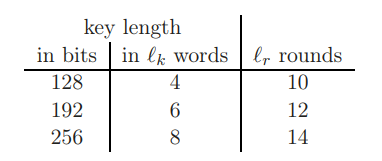
\includegraphics[width=0.5\textwidth, height=0.5\textheight, keepaspectratio]{Claves_de_AES}
        \caption{Número de palabras $l_{k}$ y de rondas $l_{r}$ de AES \cite{cryptoSchool}.}
        \label{fig:1.2}
    \end{figure}
    
    En realidad, cada palabra tiene la forma de un vector columna, simplemente $l_{k}$ indica cuantas filas componen a ese vector. En esta operación buscamos en cada ronda generar una clave de ronda, que será un vector con tantas componentes como rondas $l_{k}$ haya, más una para la ronda inicial. Por tanto, se requiere un total de $l_{k} \cdot (l_{r} + 1)$ claves de ronda.

    \begin{ejemplo}
        Por ejemplo, para una llave de $256$ bits, los mensajes consisten en $8$ palabras de $4$ bytes cada una, equivalentemente, $8$ palabras de $32$ bits cada una. Esto lo sabemos ya que a partir de la figura \ref{fig:1.2}, la clave está formada por $l_{k} = 8$ palabras del tipo $K_{0}, ... , K_{7}$. Además, sabemos que el número de rondas es $l_{r} = 14$, por lo que necesitaremos una clave extendida de $l_{k}(l_{r} + 1) = 8 \cdot (14 + 1) = 120$ palabras.
    \end{ejemplo}

    Procedemos a continuación a explicar esta operación para AES-$128$, es decir, tomando $l_{k} = 4$ y $l_{r} = 10$. La clave secreta $K$ está formada por las cuatro primeras palabras de $32$ bits $E_{0}, E_{1}, E_{2}$ y $E_{3}$ de la clave extendida $E_{0}, ... , E_{4(l_{r}+1)-1}$, que consta de $4(l_{r} + 1)$ palabras de $32$ bits. El resto se generarán a partir de las que ya tenemos. Así, nuestras claves de ronda consistirán en bloques de $4$ palabras consecutivas de la clave extendida. La forma de calcular el resto de palabras es la siguiente:
    \begin{equation}
        E_{i} = E_{i-1} + E_{i-4} \text{ , con } i \geq 4
    \end{equation}
    Esto no es más que la suma en $\mathbb{Z}_{2}^{32}$, en otras palabras, la suma de bits módulo dos o XOR, vista anteriormente. 
    
    No obstante, si $i$ es múltiplo de $4$, se aplica primero una transformación al elemento $E_{i-1}$ tal que sus elementos $(a_{0}, a_{1}, a_{2}, a_{3})$ se desplazan hacia la derecha cíclicamente, obteniendo $(a_{3}, a_{0}, a_{1}, a_{2})$. Es más, si tomamos cada palabra como un elemento $a$ de $S = \mathbb{F}_{256}[t]/(t^{4} + 1)$, consiste simplemente en multiplicar por $t^{3}$ en $S$. Despues, se aplica SubBytes a cada byte individualmente, y se añade una constante $c_{i/4}$, definida de esta forma:
    \begin{equation}
        c_{j} = (0, 0, 0, t^{j-1}) = t^{j-1} \text{ en } S
    \end{equation}
    Decimos que es una constante porque, tomandola como un elemento de $S$, tiene la forma $a_{3}t^{3} + a_{2}t^{2} + a_{1}t + a_{0}$, con $a_{3} = a_{2} = a_{1} = 0$.

    Por último, en el caso en que trabajemos con AES-$256$ y por tanto $l_k = 8$ y $l_r = 14$, se aplica otra transformación. Consiste en que $E_{i-1}$, se reemplaza por SubBytes($E_{i-1}$), si $i$ mod $8$ = $4$. Poniendo toda esta información en común, obtenemos este algoritmo explicativo:

    \begin{algorithm}[H]
        \caption{Algoritmo de clave extendida de AES}
        \textbf{Input:} Clave $K_{0}, ..., K_{l_{k}-1}$ formada por $l_{k}$ palabras, donde cada $K_{i}$ tiene $4$ bytes.\\
        \textbf{Output:} Clave extendida $E_{0}, ... , E_{l_{k}(l_{r}+1)-1}$ formada por $l_{k}(l_{r}+1)$ palabras, donde cada $E_{i}$ tiene $4$ bytes.
        \bigskip
        \begin{algorithmic}[1]
            \For{$i$ from $0$ to $l_{k}-1$}
            \State $E_{i} = K_{i}$
            \EndFor
            \For{$i$ from $l_{k}$ to $l_{k} \cdot (l_{r}+1)$}
            \State $L = E_{i-1}$
            \If{$l_{k}$ divides $i$}
            \State $c = (0, 0, 0, t^{(i/l_{k}) - 1})$
            \State $L$ = SubBytes$(s^{3} \cdot L) + c$
            \EndIf
            \If{$l_{k} == 8$ and $i$ mod $8$ == $4$}
            \State $L$ = SubBytes($L$)
            \EndIf
            \State $E_{i} = E_{i - l_{k}} + L$
            \EndFor
        \end{algorithmic}
    \end{algorithm}

    Una vez hemos descrito todas las operaciones de AES para una ronda, solo nos hace falta repetirlas en el orden y el número de veces que indica la figura \ref{fig:1.1} del principio. Aunque debemos tener en cuenta que dependiendo de qué AES estemos utilizando, el número de rondas será distinto. Con esto, damos por concluida nuestra descripción general del cifrado de AES.

    \subsection{Comentarios sobre AES}
    
    Primeramente, debemos saber que AES evolucionó a partir de los cifrados por bloques desarrollados por sus diseñadores, previos a Rijndael. Tales como ``SHARK'', desarrollado por Vincent Rijmen; y ``Square'', desarrollado por Joan Daemen. Así, su filosofía de diseño perseguía un alto nivel de rendimiento y resistencia contra el criptoanálisis lineal y diferencial.

    Como ejemplos, destacamos que para SubBytes, fué sugerida la idea de utilizar la operación de inversión, y que el módulo $m$ es el primero de los $30$ polinomios irreducibles de la Tabla C del capítulo $10$ de ``Finite Fields'' de Rudolf Lidl \& Harald Niederreiter \cite{artLidl}. MixColumns además se basa en matrices en las que cada submatriz cuadrada es no singular, una noción explicada en el teorema $8$ del capítulo $11$ de ``The theory of error-correcting codes'' de MacWilliams \& Sloane \cite{artMacSlo}.

    Asimismo, la omisión de MixColumns en la última ronda es bastante común, ya que no disminuye la seguridad (porque los bits del texto cifrado sólo se permutan de una forma públicamente conocida), pero permite el descifrado con una estructura similar.
    
    En cuanto a su rendimiento, tal y como se exige en la competición de AES, el algoritmo es rápido en una gran variedad de plataformas. Las implementaciones de software pueden alcanzar más de $12$ GB/seg. Aun así, si tenemos como objetivo realizar una implementación de software, debemos saber que generalmente es ventajoso sustituir los cálculos por consultas de tablas. Utilizando una tabla de $4$ KB, una ronda de AES puede ejecutarse con $16$ búsquedas en la tabla y $16$ XOR de $32$ bits.

    Por otro lado, en cuanto a su seguridad, sí que es cierto que algunos criptógrafos muestran preocupación, ya que sienten que el margen entre el número de rondas especificado en el cifrador y los mejores ataques conocidos es muy pequeño. Además, se especula con ataques teóricos, como por ejemplo el denominado ``Ataque XSL'', que teóricamente muestra una potencial debilidad en el algoritmo AES. Sin embargo, tanto los expertos como las instituciones de normalización más relevantes consideran que AES es seguro.

    \newpage
 
    \section{Criptografía simétrica vs asimétrica} \label{sec:1.3}

    Hasta ahora, solo hemos trabajado con AES, un criptosistema de tipo simétrico. Este tipo de criptosistemas se caracterizan porque la misma clave que se utiliza para cifrar el mensaje, es la que se usa para descifrarlo. Al igual que AES, todos los cifrados previos a $1970$ eran de este tipo. 
    
    Sin embargo, Diffie \& Hellman \cite{artDH} hicieron una propuesta revolucionaria en $1976$ publicando su libro ``New directions in cryptography'', en el que presentaron un algoritmo que demostró que la criptografía asimétrica era posible. En él, proponen un nuevo método de comunicación donde cada usuario posee dos claves, una privada y una pública. Digamos que Alice quiere enviar un mensaje a Bob. Entonces Alice debe utilizar la clave pública de Bob para encriptar el mensaje que le mandará. Gracias a la clave secreta, Bob puede fácilmente desencriptar el mensaje de Alice, pero sin ella, nadie debería poder.
    
    Con la llegada de este nuevo tipo de criptosistemas, se comenzó a estudiar si estos eran mejores o peores que los ya conocidos criptosistemas simétricos. Pero como en todo, se encontraron ventajas y desventajas en cada uno de ellos. 
    
    Por un lado, la ventaja de los criptosistemas asimétricos radica en que no necesitan un cambio de clave. Por otro, los criptosistemas simétricos tienen ventaja de velocidad, ya que como hemos mencionado, AES puede alcanzar $12$ GB/seg. Otra ventaja de estos últimos es la autenticación, puesto que en los criptosistemas asimétricos debemos tomar medidas para garantizar esta característica. 

    Actualmente, la realidad es que no existe una rivalidad entre criptografía ``Simétrica vs Asimétrica''. Por lo general, se utiliza un método asimétrico para compartir las claves necesarias y así, posteriormente, poder aplicar un criptosistema simétrico permitiendo comunicación de mayor rendimiento. 
    
    Veamos a continuación dos ejemplos de criptosistemas asimétricos para conocerlos un poco más a fondo, comenzando por el famoso criptosistema RSA.

    \section{Criptosistema RSA}

    Basándose en el primer modelo abstracto de criptosistema de clave pública sugerido por Diffie \& Hellman en $1976$, Rivest, Shamir \& Adleman crearon su propio criptosistema asimétrico en $1977$ llamado ``Rivest-Shamir-Adleman cryptosystem'', o más conocido como RSA.

    Continuemos con la notación de nombres utilizada hasta ahora. En nuestro escenario, Alice quiere enviar un mensaje a Bob, que sólo él sea capaz de leerlo. Para ello, Bob genera dos claves: una clave pública $pk$ y una clave privada $sk$. Cualquiera puede conocer la clave pública $pk$. Puede estar expuesta en una base de datos o en internet, mismamente. Sin embargo, la clave privada $sk$ sí que debe ser guardada por Bob en secreto. De esta forma, Alice usará la clave pública $pk$ para encriptar su mensaje y Bob usará su clave privada $sk$ para descifrarla.

    En los criptosistemas simétricos, el cifrado y descrifrado se realiza esencialmente con la misma clave, pero aquí, $pk$ y $sk$ son claves completamente distintas. De hecho, deben cumplir algunas propiedades como que $sk$ no debe ser computable facilmente a partir de $pk$; y deben verificar que $dec_{sk}(enc_{pk}(x)) = dec_{pk}(enc_{sk}(x)) = x$, siendo $x$ el mensaje original.

    El mensaje puede ser una imagen, un texto, un video, o incluso un programa. Pero vamos a suponer que ya ha sido convertido a un string binario (posiblemente muy largo), que será nuestra forma de comunicación estándar. Esta conversión dependerá del tipo de dato que se trate, como por ejemplo, la manera más común de enviar un texto es haciendo uso de la codificación ASCII o ASCII extendida, en letras de $7$ u $8$ bits, respectivamente. Aunque en la práctica, RSA se utiliza para enviar una clave secreta y así establecer un criptosistema simétrico; o para garantizar autenticidad mediante firmas digitales. 

    En nuestro escenario, estamos suponiendo que Alice quiere enviarle un mensaje a Bob. Para ello, Alice debe tener en cuenta el valor $n$, denominado \textit{parámetro de seguridad}, ya que debe dividir el mensaje $x$ en bloques de tamaño $n-1$ bits y enviar cada bloque por separado. Por tanto, vamos a explicar como se envía un bloque de $n-1$ bits usando el criptosistema de RSA.

    En primer lugar, Bob debe elegir dos valores primos $p$ y $q$ aleatorios, con $\frac{n}{2}$ bits cada uno. Así, su producto $N = p \cdot q$ tendrá $n$ bits. Además, Bob debe elegir un número entero $e$ aleatorio, tal que $1 \leq e < N$ y gcd($e, (p-1)(q - 1)) = 1$, es decir, $e$ y el producto $(p-1) \cdot (q-1)$ sean coprimos. Así, la clave pública de Bob es $pk = (N, e)$. 

    A continuación, a partir del mensaje $x$, Alice envía a Bob el mensaje encriptado $y = x^{e}$ en $\mathbb{Z}_{n}$, esto es, el resto de dividir $x^{e}$ entre $N$. La magia es que Bob ahora puede recuperar el mensaje de Alice $x$ con la ayuda de su información secreta relativa a $(p,q)$. El algoritmo es el siguiente:

    \begin{algorithm}[H]
        \caption{Algoritmo de generación de claves de RSA}
        \textbf{Input:} Parámetro de seguridad $n$.\\
        \textbf{Output:} Clave privada $sk$ y clave pública $pk$.
        \bigskip
        \begin{algorithmic}[1]
            \State Elegir los valores primos $p$, $q$ tal que $2^{(n-1)/2} < p$ y $q < 2^{n/2}$.
            \State Calcular $N = p \cdot q$ con $n$ bits y $L = (p - 1) \cdot (q - 1) = \phi(p) \cdot \phi(q) = \phi(N)$, es decir, la función de Euler aplicada a $N$.
            \State Escoger $e$ de manera uniformemente aleatoria del conjunto $\{2, ... , L-2\}$, tal que sea coprimo con $L$. Así $e \in \mathbb{Z}_{L}$.
            \State Calcular el inverso $d$ de $e$ en $\mathbb{Z}_{L}$. Así $d \in \mathbb{Z}_{L}$.
            \State Revelar la clave pública $pk = (N, e)$ y esconder la clave privada $sk = (N, d)$.
        \end{algorithmic}
    \end{algorithm}

    \begin{algorithm}[H]
        \caption{Algoritmo de cifrado de RSA}
        \textbf{Input:} Mensaje $x \in \mathbb{Z}_{N}$ y clave pública $pk = (N, e)$.\\
        \textbf{Output:} Mensaje cifrado $y = enc_{pk}(x) \in \mathbb{Z}_{N}$.
        \bigskip
        \begin{algorithmic}[1]
            \State Aplicar la transformación $y = x^{e}$ en $\mathbb{Z}_{N}$.
            \State Devolver el mensaje cifrado $y = enc_{pk}(x)$.
        \end{algorithmic}
    \end{algorithm}
    
    \begin{algorithm}[H]
        \caption{Algoritmo de descifrado de RSA}
        \textbf{Input:} Mensaje cifrado $y \in \mathbb{Z}_{N}$ y clave privada $sk = (N, d)$.\\
        \textbf{Output:} Mensaje original $x = dec_{sk}(y) \in \mathbb{Z}_{N}$.
        \bigskip
        \begin{algorithmic}[1]
            \State Aplicar la transformación $x = y^{d}$ en $\mathbb{Z}_{N}$.
            \State Devolver el mensaje original $x = dec_{sk}(y)$.
        \end{algorithmic}
    \end{algorithm}
    
    \begin{ejemplo} \label{ej: 1.11}
        Veamos un ejemplo tomando $n = 6$. Si en este caso comprobamos las condiciones de manera literal, debemos escoger números primos entre $6$ y $7$, pero al ser valores tan pequeños, tomaremos la libertad de ser un poco más liberales y escogeremos $p = 7$ y $q = 11$. Así, $N = 77$ y $L = 60$. Tomando $e = 17$ y aplicando el Algoritmo Extendido de Euclides, obtenemos que $d = e^{-1} = 53$ en $\mathbb{Z}_{60}$. De esta forma, Bob ya puede publicar su clave pública $pk = (77, 17)$ y guardar su clave privada $sk = (77, 53)$.

        Posteriormente, Alice quiere mandarle un mensaje a Bob, pongamos $x = 10 = (00001010)$. Entonces Alice debe cifrar el mensaje $y = x^{e} = 10^{17}$ en $\mathbb{Z}_{77}$. La forma intuitiva para calcular esto sería computar $10^{17}$ y aplicarle el módulo $77$. Pero esto tiene un problema, y es que para valores reales de $n$, $x^{e}$ puede superar el número de partículas en el universo. Sin embargo, hay una forma más sencilla de calcularlo. La idea es descomponer el valor en sus potencias de dos y aplicar módulo tras cada operación para no dejar que el valor se dispare. Veamoslo:
        \begin{align}
            \text{Ya q} & \text{ue }(17)_{10} = (10001)_{2} \Rightarrow 10^{17} = 10^{2^{0}+2^{4}} = 10 \cdot 10^{16} \\
            \text{Calc} & \text{ulamos} \text{ así las potencias de $10$ mod $77$:} \\
            &10 \text{ mod } 77 = 10 \\
            &10^{2} \text{ mod } 77 = 10 \cdot 10 \text{ mod } 77 = 23 \\
            &10^{4} \text{ mod } 77 = 10^{2} \cdot 10^{2} \text{ mod } 77 = 23^{2} \text{ mod } 77 = 67 \\
            &10^{8} \text{ mod } 77 = 10^{4} \cdot 10^{4} \text{ mod } 77 = 67^{2} \text{ mod } 77 = 23 \\
            &10^{16} \text{ mod } 77 = 10^{8} \cdot 10^{8} \text{ mod } 77 = 23^{2} \text{ mod } 77 = 67 \\
            \text{Por } & \text{tanto,} \\
            &10^{17} \text{ mod } 77 = 10 \cdot 10^{16} \text{ mod } 77 = 10 \cdot 67 \text{ mod } 77 = 54
        \end{align}
        Ahora, Alice ya puede enviar su mensaje cifrado $y = enc_{pk}(10) = 54$ a Bob. Por tanto, Bob debe descifrar el mensaje recibido, y para ello, debe usar de manera análoga la descomposición binaria de $53$ (que es el valor de su clave secereta $sk$) para descifrar el mensaje en $\mathbb{Z}_{77}$. De esta forma, $dec_{sk}(54) = x = 54^{53} = 10$ en $\mathbb{Z}_{77}$. De hecho, ese es el mensaje original que Alice quería hacerle llegar a Bob.
    \end{ejemplo}
    
    \begin{observacion}
        Tal y como ya hemos mencionado antes, debemos dejar claro que los valores tomados en este ejemplo son simplemente para esclarecer las ideas del método propuesto, ya que con objetivos prácticos reales, es recomendable que el valor del parámetro de seguridad sea mayor a $n = 3000$.
    \end{observacion}

    \section{Intercambio de claves Diffie-Hellman}

    Para los criptosistemas simétricos como AES, se debe elegir una clave secreta y compartirla entre todos las partes autorizadas. En la práctica, este acuerdo plantea una gran dificultad en este tipo de criptosistemas. Para ilustrar esto, comenzaremos esta sección con un ejemplo histórico.

    Durante la Primera Guerra Mundial, los alemanes quedaron aislados de sus embajadas en el extranjero. Surgieron las sospechas de que sus antiguos códigos de comunicación estaban rotos y enviaron un código nuevo a México y a Washington en un submarino. Sin embargo, esta clave no pudo ser entregada con éxito a México. A pesar de esto, un mensaje secreto de gran importancia llegó sin problemas a Washington utilizando el nuevo código, aunque, posteriormente tuvo que ser retransmitido a México en el código antiguo, el cual fue descifrado. La implementación en su momento de un método público y seguro para el intercambio de claves secretas podría haber evitado esta situación.

    Por tanto, la pregunta es la siguiente: ¿Pueden dos usuarios ponerse de acuerdo sobre una clave secreta compartida (para un criptosistema simétrico) mientras se ven obligados a utilizar un canal inseguro? La sorprendente respuesta es que sí es posible. Obviamente, ninguno puede enviar directamente la clave secreta ya que el canal es inseguro. En lugar de eso, cada usuario debe enviar una versión enmascarada de la clave, a partir de la cual el otro usuario pueda obtenerla, pero un espía no pueda.

    Diffie y Hellman proponen el uso de un número primo $p$, y a partir de él, trabajar con valores que no sean divisibles por $p$ y las propiedades de su producto. Estos valores forman el grupo $\mathbb{Z}_{p}^{x}$ de unidades módulo $p$. En total hay $p - 1$ elementos y el producto de dos de ellos tampoco es divisible por $p$. Además, todos los elementos tienen inverso multiplicativo, que se puede calcular haciendo uso del Algoritmo Extendido de Euclides. Asimismo, este grupo $G = \mathbb{Z}_{p}^{x}$ es \textit{cíclico}, esto es, que existe un elemento $g \in G$, llamado \textit{generador}, cuyas potencias generan todos los elementos de $G = \{g^{0} = 1, g, g^{2}, ... , g^{p-2}\} = \langle g \rangle$. El \textit{orden} del grupo, es decir, el número de elementos de $G$, lo denotaremos como $d$. Aparece ahora un parámetro de seguridad global $n$, que indica el tamaño de $d$ en bits. Así, los elementos de $G$ pueden representarse por cadenas de $n$ bits.

    Un requisito importante es que la representación de $G$ pueda ser expresada utilizando una cantidad de bits que crezca de manera polinómica respecto al valor $n$. Otro requisito, es que las operaciones del grupo puedan transformarse en las representaciones de los elementos de $G$, con una cantidad de operaciones que aumente de manera polinómica respecto a $n$. En general, estos dos requisitos se cumplen de manera clara.

    Algunos ejemplos de $G$ son los siguientes:
    \begin{itemize}
        \item El grupo multiplicativo $G = \mathbb{Z}_{p}^{x}$ de unidades módulo $p$.
        \item El grupo multiplicativo $G = \mathbb{F}_{q}^{x}$ de un cuerpo finito $\mathbb{F}_{q}$.
        \item Grupos cíclicos de curvas elípticas sobre cuerpos finitos.
    \end{itemize}
    
    \begin{ejemplo} \cite{cryptoSchool}
        Sea $G = \mathbb{Z}_{2579}^{x}$ el grupo multiplicativo de unidades módulo $p = 2579$. Como $d = \phi(2579) = 2578 = 2 \cdot 1289$, con $2$ y $1289$ primos, y $2^{2} = 4$ y $2^{1289} = -1$ en $\mathbb{Z}_{2579}^{x}$, ambos distintos de $1$, concluimos que $g = 2 \in G$ es el generador de $G$. Una descripción de $G$ equivale a unos bits diciendo: ``$G$ es de la forma $\mathbb{Z}_{p}^{x}$''. Entonces, $G$ es identificado como el conjunto $\{0, ... , p-1\}$ y la representación binaria de los enteros proporciona la representación de los elementos de $G$. En este ejemplo, tomando $n = 12$, ciertas herramientas para aritmética eficiente muestran que las operaciones de grupo pueden realizarse con coste cuadrático, y por tanto, polinómico en $n$.
    \end{ejemplo}

    Procedemos a describir el intercambio de claves de Diffie-Hellman basándonos en la siguiente representación gráfica.
    
    \begin{figure}[H]
        \centering
        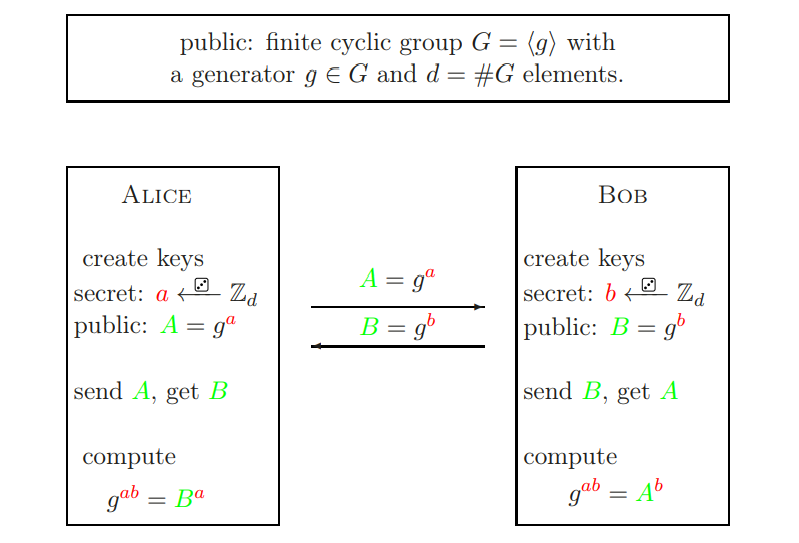
\includegraphics[width=0.8\textwidth, height=0.8\textheight, keepaspectratio]{RepresentacionDH}
        \caption{Esquema del intercambio de claves Diffie-Hellman \cite{cryptoSchool}.}
    \end{figure}

    En primer lugar, Alice y Bob deben elegir de forma independiente una clave secreta aleatoria $a$ y $b \in \mathbb{Z}_{d}$. A continuación, ambos publican sus claves públicas $A = g^{a}$ y $B = g^{b}$, respectivamente. Ahora, ambos pueden calcular, tal vez para su uso en un criptosistema de clave simétrica, la clave secreta compartida $g^{ab}$:
    \begin{equation}
        g^{ab} = B^{a} = A^{b}
    \end{equation}
    ya que
    \begin{equation}
        B^{a} = (g^{b})^{a} = g^{ba} = g^{ab} = (g^{a})^{b} = A^{b}
    \end{equation}
    
    El algoritmo es el siguiente:
 
    \begin{algorithm}[H]
        \caption{Intercambio de claves Diffie-Hellman}
        \textbf{Input:} Parámetro de seguridad $n$.\\
        \textbf{Output:} $G, g, d$ explicadas y clave secreta compartida $k_{B} = k_{A} = g^{ab}$.
        \bigskip
        \begin{algorithmic}[1]
            \State Describir un grupo cíclico finito $G = \langle g \rangle$, siendo $g$ su generador y con $d = \#G$ elementos, donde $d$ es un entero de $n$ bits.
            \State Alice elige su clave secreta $sk = a \in \mathbb{Z}_{d}$, y publica su clave pública $pk = A = g^{a} \in G$.
            \State Bob elige su clave secreta $sk = b \in \mathbb{Z}_{d}$, y publica su clave pública $pk = B = g^{b} \in G$.
            \State Alice y Bob intercambian sus claves públicas $A$ y $B$.
            \State Alice obtiene su clave secreta compartida $k_{A} = B^{a}$ en $G$.
            \State Bob obtiene su clave secreta compartida $k_{B} = A^{b}$ en $G$.
            \State Alice y Bob tienen ahora sus claves secretas compartidas $k_{B} = k_{A}$.
        \end{algorithmic}
    \end{algorithm}

    \begin{ejemplo} \cite{cryptoSchool}
        Continuamos con el ejemplo tratado anteriormente. Podemos así seguir con exactitud los pasos vistos en el algoritmo de intercambio de claves:
        \begin{algorithmic}[1]
            \State Recordemos que estábamos trabajando con $G = \mathbb{Z}_{2579}^{x}$ y cuyo generador es $g = 2 \in G$.
            \State Alice elige su clave secreta $sk = a = 765 \in \mathbb{Z}_{d}$, y publica su clave pública $pk = A = g^{a} = 2^{765} = 949 \in G$.
            \State Bob elige su clave secreta $sk = b = 853 \in \mathbb{Z}_{d}$, y publica su clave pública $pk = B = g^{b} = 2^{853} = 435 \in G$.
            \State Alice y Bob intercambian sus claves públicas $A = 949$ y $B = 435$.
            \State Alice obtiene su clave secreta compartida $k_{A} = B^{a} = 435^{765} = 2424 \in G$.
            \State Bob obtiene su clave secreta compartida $k_{B} = A^{b} = 949^{853} = 2424 \in G$.
            \State Alice y Bob tienen ahora sus claves secretas compartidas $k_{B} = k_{A} = 2424 \in G$.
        \end{algorithmic}
    \end{ejemplo}

    \begin{observacion}
        Como ya hemos mencionado, el método es correcto, en cuanto a que tanto Bob como Alice obtienen la misma clave secreta compartida que les permite generar un cifrado simétrico para comunicarse, entre otras cosas. Por otro lado, en cuanto a eficiencia, la operación más costosa es la exponenciación en $G$, pero justo en el apartado anterior de RSA explicamos una forma de realizar esta operación de manera mucho más eficiente, específicamente en el ejemplo \ref{ej: 1.11}. Por último, el principal problema que tiene este método en cuanto a seguridad, es el ataque conocido como \textit{man-in-the-middle} (MITM). En nuestro caso, este ataque consiste en que Eva se hace pasar por Alice cuando habla con Bob y por Bob cuando intercambia datos con Alice. Ambas partes creen que al otro lado tienen a la pareja legítima, pero Eva puede actuar de forma maliciosa generando su propia parte de la clave compartida utilizada. Para solucionar esto, pueden simplemente comparar si las claves secretas compartidas son idénticas. Si no lo son, pueden estar seguros de que alguien ha estado interfiriendo en su comunicación.
    \end{observacion}

    Para finalizar, debemos destacar que en la actualidad, el protocolo Diffie-Hellman se emplea en situaciones prácticas ampliamente reconocidas. Un ejemplo de su uso es el protocolo de mensajería instantánea conocido como \textit{Off-the-Record Messaging} (OTR). Además, se utiliza en la red de anonimato denominada \textit{Tor}, donde el protocolo Diffie-Hellman se implementa sobre una conexión TLS previamente establecida en una capa inferior. Esta implementación se utiliza para generar claves de sesión entre el cliente y los nodos de enrutamiento de la red, y estas claves se emplean para cifrar las capas de cebolla de los paquetes que circulan a través de la red.
    
\endinput